% {{{ Packages

% {{{ Versions
% version écran
\documentclass{beamer}

% version orateur
%\setbeameroption{show only notes}
%\usepackage{pgfpages}
%\pgfpagesuselayout{2 on 1}[a4paper,border shrink=5mm]

% version spectateur
%\documentclass[handout]{beamer}
%\usepackage{handoutWithNotes}
%\pgfpagesuselayout{1 on 1 with notes}[a4paper,border shrink=5mm]
% }}}

\usepackage[utf8]{inputenc}
\usepackage[french]{babel}
\usepackage{tikz}
\usepackage{caption}
\usepackage{listings}
\usetheme[numbering=none]{metropolis}

% }}}
% {{{ Commands
\makeatletter
\def\ft@overlay{}

\addtobeamertemplate{footline}{}
{
    \lineskiplimit0pt
    \begin{tikzpicture}[remember picture,overlay]
        \ft@overlay
    \end{tikzpicture}
    \gdef\ft@overlay{}
}

\newcommand<>{\addtooverlay}[1]{
    \only#2{
      \expandafter\gdef\expandafter\ft@overlay\expandafter{\ft@overlay
          \draw[fill=black,opacity=0.70]
              (current page.north east) rectangle (current page.south west);
          \node[text=white] at (current page.center) {
              #1
          };
      }
    }
    \pause
}
% }}}

\title{Étendre composer}
\author{Nicolas \textsc{Joseph}}
\date{28 octobre 2016}
\institute{Forum PHP}

\begin{document}
% {{{ Titre
\begin{frame}
    \titlepage
\end{frame}
\note {
    Bonjour à tous,

    J’imagine que vous commencez à voir faim, je vais donc faire vite.
}
% }}}
% {{{ Les nouvelles commandes
\section{Les nouvelles commandes}
\begin{frame}
    \frametitle{Les nouvelles commandes}

    \addtooverlay<.(1)>{
        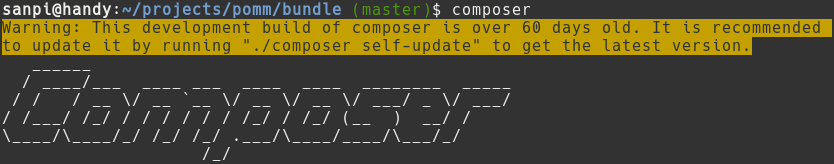
\includegraphics[scale=0.28]{images/update}
    }
\end{frame}

\note {
    Mais avant d’aborder le sujet de cette présentation, je voudrais revenir sur
    les nouveautés de composer.

    Enfin, nouveautés qui ont environ deux ans, car si comme moi, vous vous
    contentez de faire un `self-update` tous les deux mois, vous êtes
    probablement passé à côté de pas mal de commandes fort sympatiques.
}

\begin{frame}
    \frametitle{Les nouvelles commandes}

    \begin{itemize}[<+->]
        \item license
        \addtooverlay<.(1)>{
            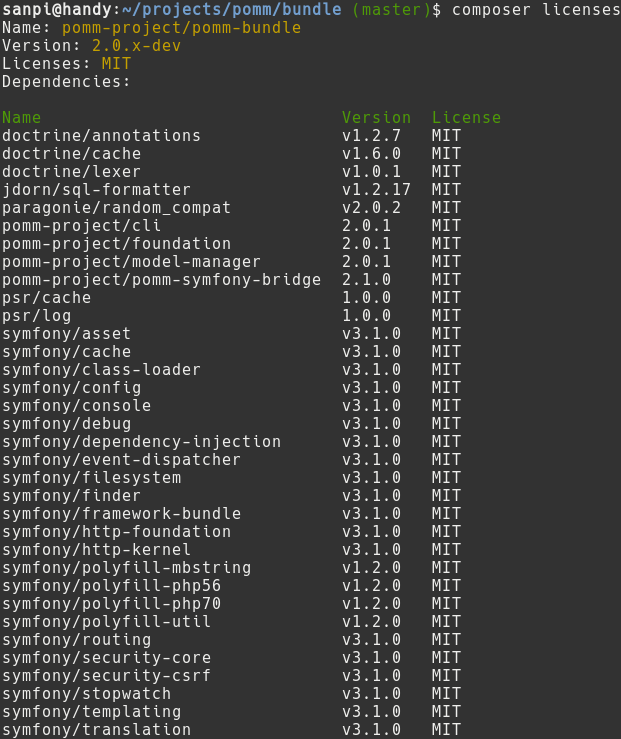
\includegraphics[scale=0.28]{images/licenses}
        }

        \item suggests
        \addtooverlay<.(1)>{
            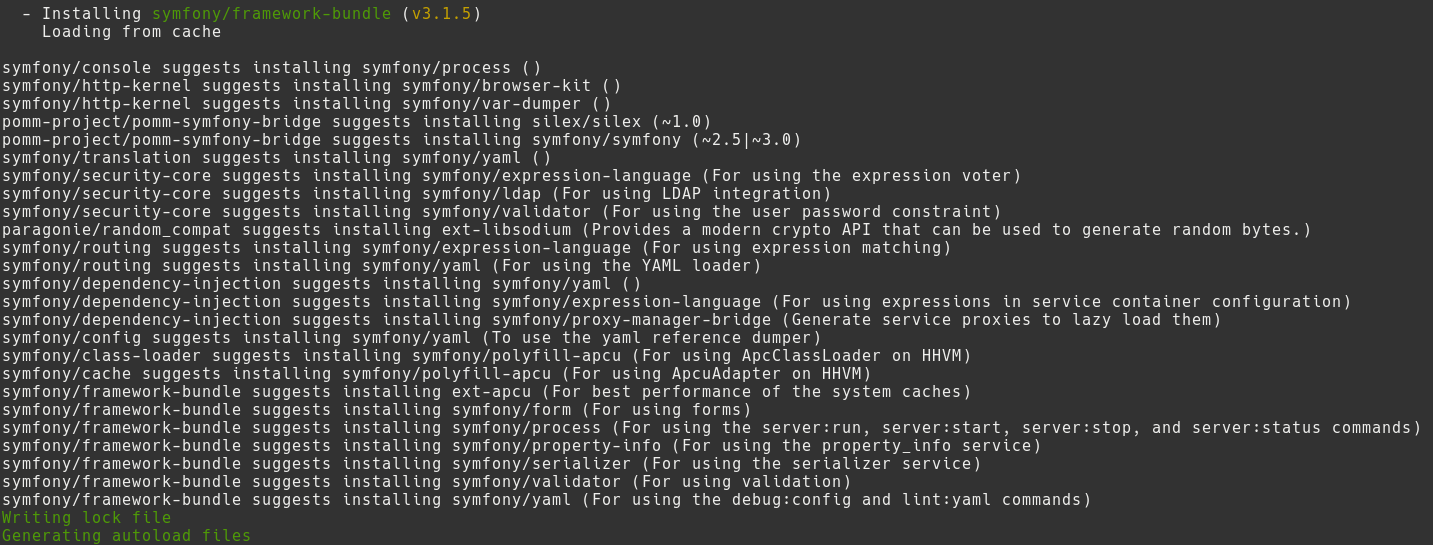
\includegraphics[scale=0.21]{images/suggests-install}
        }

        \addtooverlay<.(1)>{
            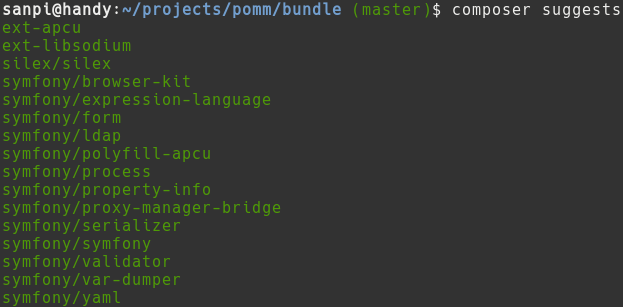
\includegraphics[scale=0.28]{images/suggests}
        }

        \item outdated
        \addtooverlay<.(1)>{
            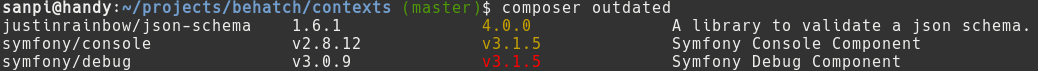
\includegraphics[scale=0.28]{images/outdated}
        }

        \item why
        \addtooverlay<.(1)>{
            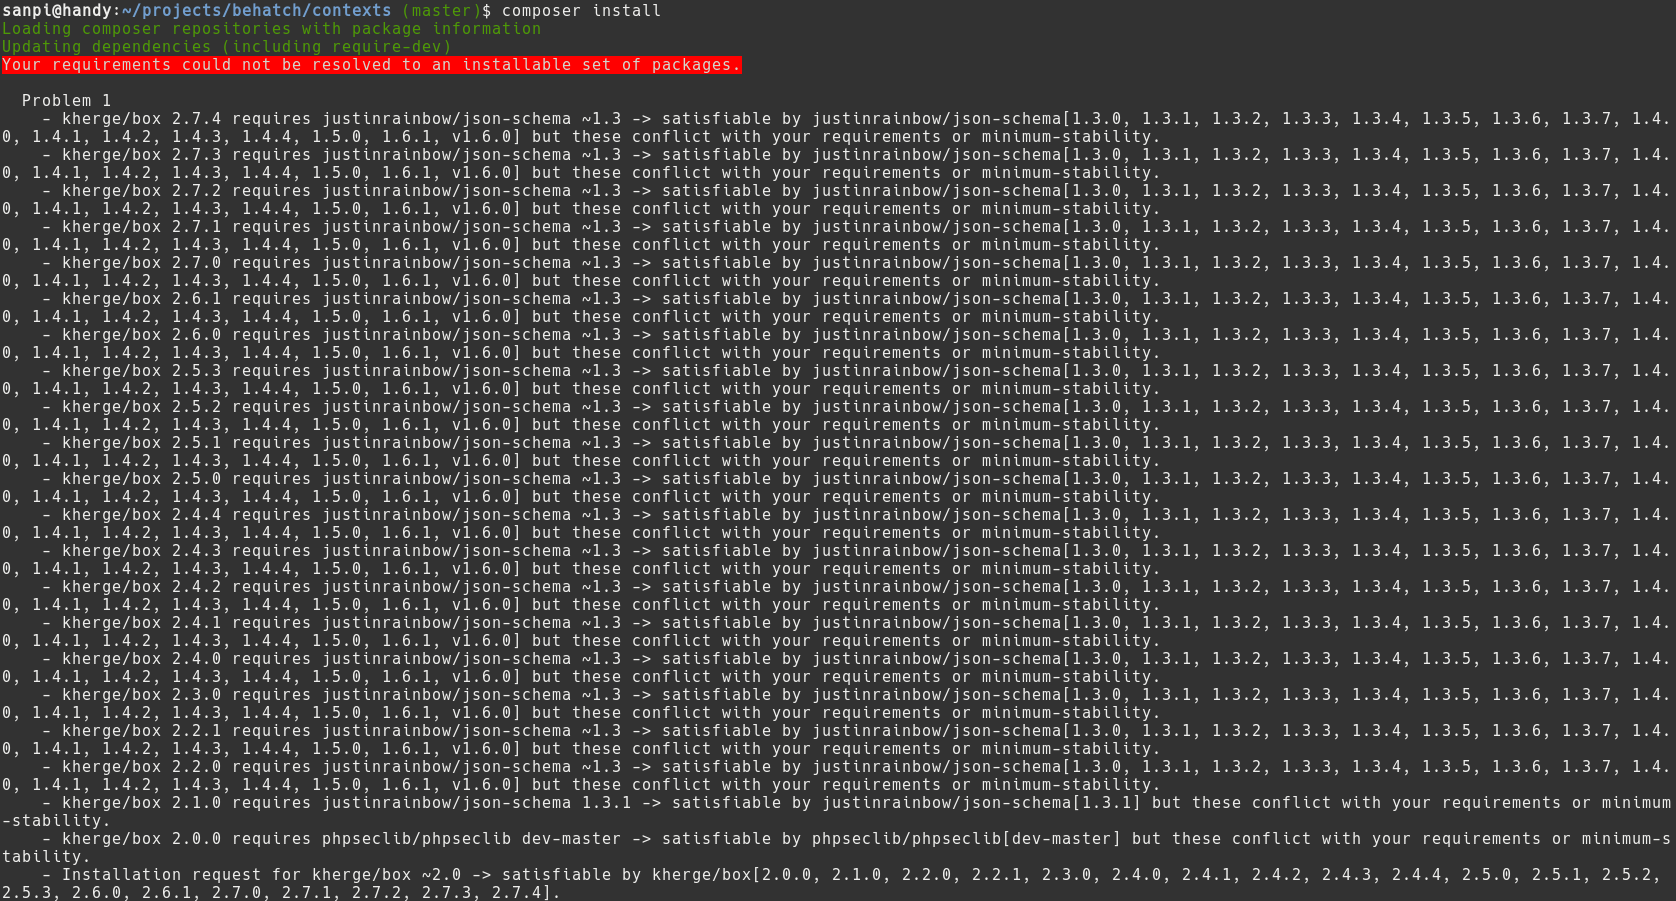
\includegraphics[scale=0.21]{images/conflict}
        }

        \addtooverlay<.(1)>{
            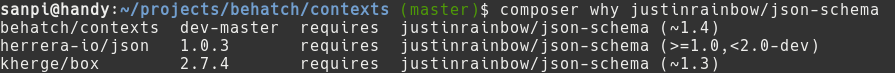
\includegraphics[scale=0.28]{images/why}
        }
    \end{itemize}
\end{frame}

\note {
    Donc quelques « nouvelles » commandes.

    Une autre commande, aussi simple, permet de rapidement lister les
    licenses des dépendances.

    Dans vos paquets, vous pouvez suggérez d’autres dépendances que vos
    utilisateurs peuvent installer. Avant, cette liste était affichée après un
    composer install de manière peu claire. Et puis je viens de faire une
    installation, ce n’est pas à ce moment que je vais chercher d’autre paquet à
    installer. Par contre plus tard, lors de l’implémentation d’une nouvelle
    fonctionnalité, vous pouvez retrouver cette liste qui peux être un bon point
    de départ.

    Bon, passons à quelque chose de plus instéressant afin d’arrêter
    de lancer un composer update à l’aveugle et d’avoir un aperçu de ce qu’il va
    se passer.

    Et pour finir, une commande qui devrait grandement vous aider en vous
    affichant clairement pourquoi tel paquet est installé avec tel version.
}

\begin{frame}
    \frametitle{Les nouvelles commandes}

    \url{https://github.com/composer/composer/releases.atom}
    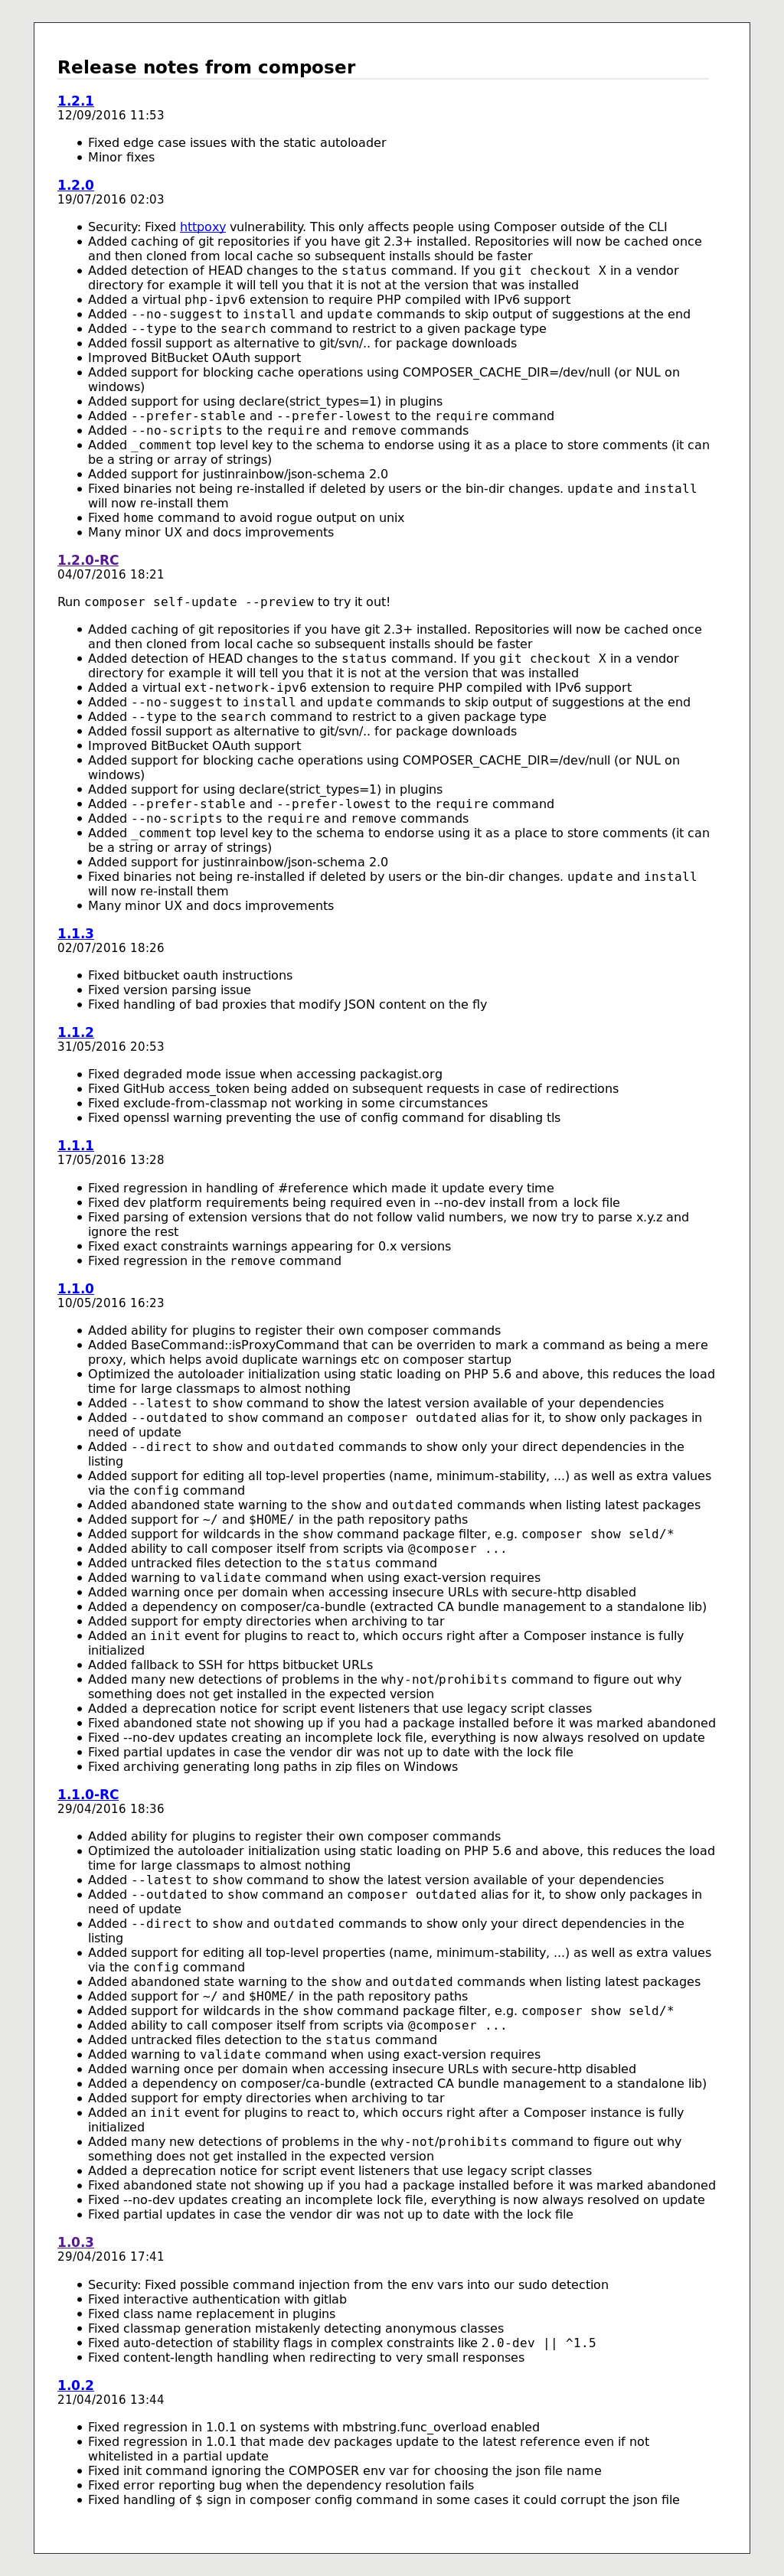
\includegraphics[scale=0.28]{images/releases}
\end{frame}

\note {
}
% }}}
% {{{ Les scripts
\section{Les scripts}

\begin{frame}
    \frametitle{Les scripts}

    \addtooverlay<.(1)>{
        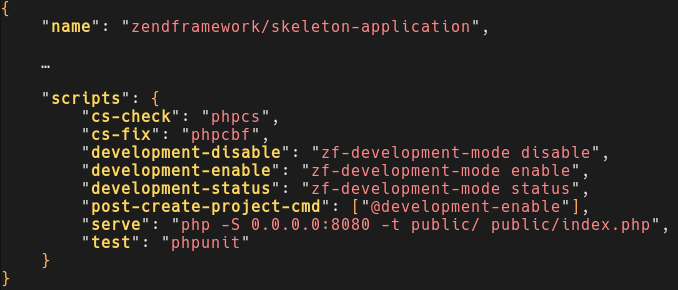
\includegraphics[scale=0.28]{images/composer/zf}
    }

    \addtooverlay<.(1)>{
        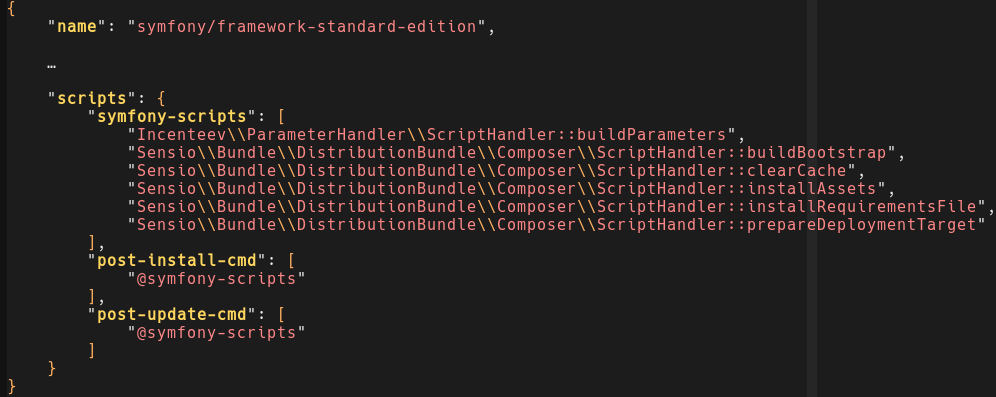
\includegraphics[scale=0.28]{images/composer/sf}
    }
\end{frame}

\note {
    Bon il est temps d’entrer dans le cœur de cette présentation, avec une
    première méthode d’étendre composer. Les scripts. Vous connaissez
    probablement cette méthode puisqu’elle est utilisée par les frameworks les
    plus connus :

    Zend, qui se contente de proposer des alias pour des commandes bash.

    Autre possibilité, utilisée par symfony, est de passer par une méthode php.
    Notez au passage l’utilisation d’alias pour éviter de répéter les commandes.
}

\begin{frame}
    \frametitle{Les scripts}

    \begin{columns}
        \begin{column}{6cm}
            \begin{itemize}
                \item Command events
                \begin{itemize}
                    \item \{pre,post\}-install-cmd
                    \item \{pre,post\}-update-cmd
                    \item \{pre,post\}-status-cmd
                    \item \{pre,post\}-archive-cmd
                    \item \{pre,post\}-autoload-cmd
                    \item \{pre,post\}-root-package-cmd
                \end{itemize}

                \item Installer events
                \begin{itemize}
                    \item \{pre,post\}-dependencies-solving
                \end{itemize}
            \end{itemize}
        \end{column}

        \begin{column}{6cm}
            \begin{itemize}
                \item Package events
                \begin{itemize}
                    \item \{pre,post\}-package-install
                    \item \{pre,post\}-package-update
                    \item \{pre,post\}-package-uninstall
                \end{itemize}

                \item Plugin events
                \begin{itemize}
                    \item init
                    \item command
                    \item pre-file-download
                \end{itemize}
            \end{itemize}
        \end{column}
    \end{columns}
\end{frame}

\note {
    Dans tous les cas, voici un aperçu des accroches possibles. Je vous laisse
    les regarder pendant que je me désaltère.
}
% }}}
% {{{ Les plugins
\section{Les plugins}

\note {
    Bon il est temps d’entrer dans le cœur de cette présentation : les plugins.
}

\begin{frame}
    \frametitle{Qu’est ce qu’un plugin ?}
\end{frame}

\note {
    Comment créer un plugin.
}

\begin{frame}
    \frametitle{Qu’est ce qu’un plugin ?}

    \begin{itemize}[<+->]
        \item type: "composer-plugin"
        \item require: \{ "composer-plugin-api": "\^{}1.0" \}
        \item extra: \{ "class": "My$\backslash$Plugin" \}
    \end{itemize}
\end{frame}

\note[itemize] {
    \item Il suffit de *créer* un projet de type *composer-plugin*.
    \item De dépendre de l’api composer.
    \item Et enfin de préciser la classe qui sera le point d’entrée du plugin.
}

\begin{frame}
    \frametitle{Qu’est ce qu’un plugin ?}

    \begin{itemize}[<+->]
        \item Composer$\backslash$Plugin$\backslash$PluginInterface
        \addtooverlay<.(1)>{
            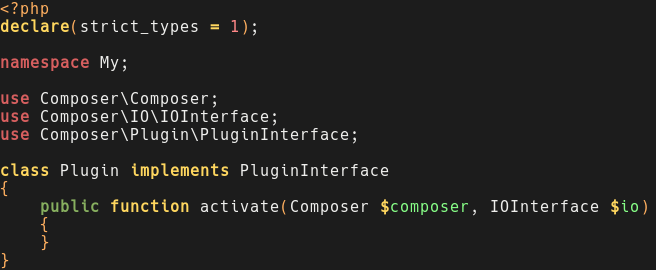
\includegraphics[scale=0.28]{images/activate}
        }

        \item Composer$\backslash$EventDispatcher$\backslash$EventSubscriberInterface
        \addtooverlay<.(1)>{
            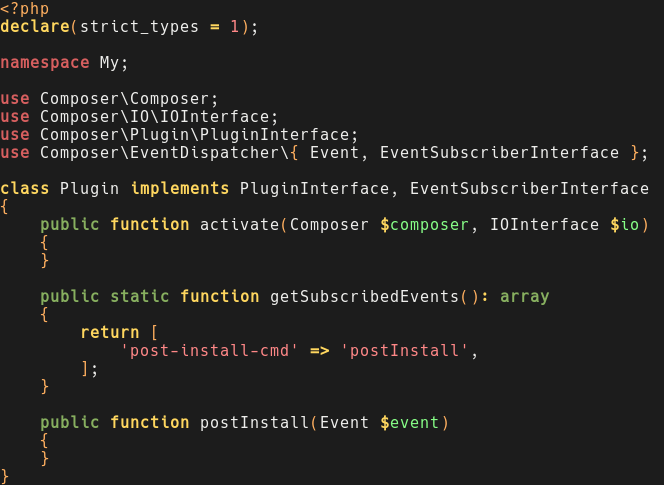
\includegraphics[scale=0.28]{images/event-subscriber}
        }

        \item Composer$\backslash$Plugin$\backslash$Capable

        \item Composer$\backslash$Plugin$\backslash$Capability$\backslash$CommandProvider
        \addtooverlay<.(1)>{
            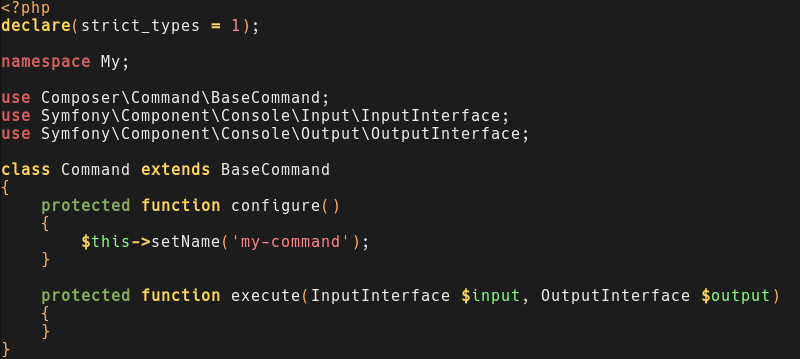
\includegraphics[scale=0.28]{images/command}
        }
    \end{itemize}
\end{frame}

\note[itemize] {
    \item Cette classe doit implémenter l’interface PluginInterface.
    \item Qui nécessite une seule méthode activate qui sera appelée à chaque
        commande lancée. Vous aurez accès à la une instance de la classe
        Composer.
    \item Il existe églament l’interface EventSubscriberInterface, qui va
        fortement ressembler au scripts que l’on a vu précédemment.
    \item L’interface Capable est simplement là pour réduire le coupage à la
        classe Composer, je passe dessus.
    \item Et enfin CommandProvider, va permettre de créer de nouvelles
        commandes.
}

\begin{frame}
    \frametitle{Où les trouver ?}
\end{frame}

\begin{frame}
    \frametitle{Où les trouver ?}

    \begin{itemize}[<+->]
        \item \small \url{https://packagist.org/search/?q=composer-plugin-api}
        \item \small \url{https://packagist.org/packages/list.json?type=composer-plugin}
    \end{itemize}
\end{frame}

\note[itemize] {
    \item Maintenant que vous avez une bonne idée de ce qu’il est possible de
        faire avec un plugin, où les trouver ?
    \item Bien évidemment sur packagist, mais au bout de quelques pages, la
        recherche remonte n’importe quoi.
    \item Du coup vous pouvez passer par l’API, mais c’est mois pratique à lire…
}

\begin{frame}
    \frametitle{Quelques plugins}
\end{frame}

\begin{frame}
    \frametitle{Quelques plugins}

    \begin{itemize}[<+->]
        \item hirak/prestissimo
        \item fxp/composer-asset-plugin
        \item stecman/composer-bash-completion-plugin
        \item netresearch/composer-patches-plugin
    \end{itemize}
\end{frame}

\note[itemize] {
    \item Pour finir, quelques plugins qui risque rapidement de devenir
        indispensable.
    \item prestissimo, pour l’annectot c’est le premier que j’ai découvert et
        c’est en cherchant comment il fonctionnait que j’ai découvert tout ce
        que je viens de vous raconter. Donc prestissimo va tout simplement
        parralelliser le téléchargement des dépendances.
    \item composer-asset-plugin, permet d’installer des dépendances npm ou bower
        via composer.
    \item composer-bash-completion-plugin, indispensable pour obtenir
        l’autocompletion sous bash
    \item composer-patches-plugin, celui-là je ne sais pas si c’est une bonne
        idée. Il permet d’appliquer un patch aux dépendances, plutôt que de
        maintenir un fork. Si le plugin n’est pas installé sur la machine de
        déploiement, le patch ne sera pas appliqué sans message d’erreur.
}
% }}}
% {{{ Références
\section{Références}
\begin{frame}
    \frametitle{Références}

    \begin{itemize}
        \item \small \url{https://getcomposer.org/doc/articles/scripts.md}
        \item \small \url{https://getcomposer.org/doc/articles/plugins.md}
    \end{itemize}
\end{frame}
% }}}
% {{{ Questions
\begin{frame}
    \frametitle{Questions ?}

    \begin{figure}
        
\includegraphics{images/qrcode}
        \captionsetup{labelformat=empty}
        \caption{
            \href{https://github.com/sanpii/slides/releases/download/forum-php/composer-plugins.pdf}
                {github.com/\textbf{\alert{sanpii/slides}}}
        }

        \href{https://legacy.joind.in/talk/view/19053}
            {legacy.joind.in/talk/view/19053}
        \href{http://lanyrd.com/2016/forumphp/sfkhpx/}
            {lanyrd.com/2016/forumphp/sfkhpx}
    \end{figure}
\end{frame}
% }}}
\end{document}
